\documentclass[11pt]{article}
\usepackage{graphicx}
\usepackage[margin=2.5cm]{geometry}
\usepackage{tikz}
\usepackage{indentfirst}
\usepackage{tabularx}
\usepackage{listingsutf8}
\usepackage{color}
\usepackage{hyperref}
\usepackage[portuguese]{babel}

\graphicspath{{./images/}}

\lstset{
	belowcaptionskip=1\baselineskip,
	captionpos=b,
	frame=tb,
	language=c,
	aboveskip=3mm,
	belowskip=3mm,
	showstringspaces=false,
	columns=flexible,
	basicstyle={\small\ttfamily},
	numbers=none,
	numberstyle=\tiny\color{gray},
	keywordstyle=\color{blue},
	commentstyle=\color{dkgreen},
	stringstyle=\color{mauve},
	breaklines=true,
	breakatwhitespace=true,
	tabsize=3,
	inputencoding=utf8,
	extendedchars=true,
	literate={á}{{\'a}}1 {ã}{{\~a}}1 {à}{{\`a} }1 {Ã}{{\~A}}1 {ó}{{\'o}}1 {Ó}{{\'O}}1 {Í}{{\'I}}1 {í}{{\'i}}1 {é}{{\'e}}1 {ç}{{\c{c}}}1 {Ç}{{\c{C}}}1 {ú}{{\'u}}1 {õ}{{\~o}}1
}

\begin{document}
	\begin{titlepage}
    	\begin{center}
    		
\includegraphics[width=0.6\textwidth]{logo-isec}
    		
    		\vspace*{\fill}
    		
    		\Huge
    		\textbf{Tecnologias de Ligação}
    		
    		\huge
    		Projeto de planeamento e configuração de uma rede
    		
    		\vspace{0.5cm}
    		\LARGE
    		2021 - 2022
    		
    		\vspace{1.5cm}
    		
    		\textbf{Bruno Teixeira - 2019100036}
    		
    		\vfill
    		\vspace*{\fill}
    		
    		\normalsize
    		Licenciatura em Engenharia Informática \\
    		30 de janeiro de 2022		
    	\end{center}
    \end{titlepage}
	


	\tableofcontents
	\pagebreak
	\listoffigures
	\pagebreak
	
	\large	
	\section{Introdução}
	\normalsize
	\paragraph{}
	Este trabalho tem como objetivo o planeamento de uma rede de dados alargada e distríbuida de uma organização fictícia com o intuito de alargar a competência do aluno no que toca a planeamento do projeto, desenho e implementação de redes locais e alargadas e respetiva configuração de routers baseados no sistema operativo Cisco IOS/IOU.
    
	\large
	\section{Topologia}
	\normalsize
	
	\begin{figure}[h]
		\centering
		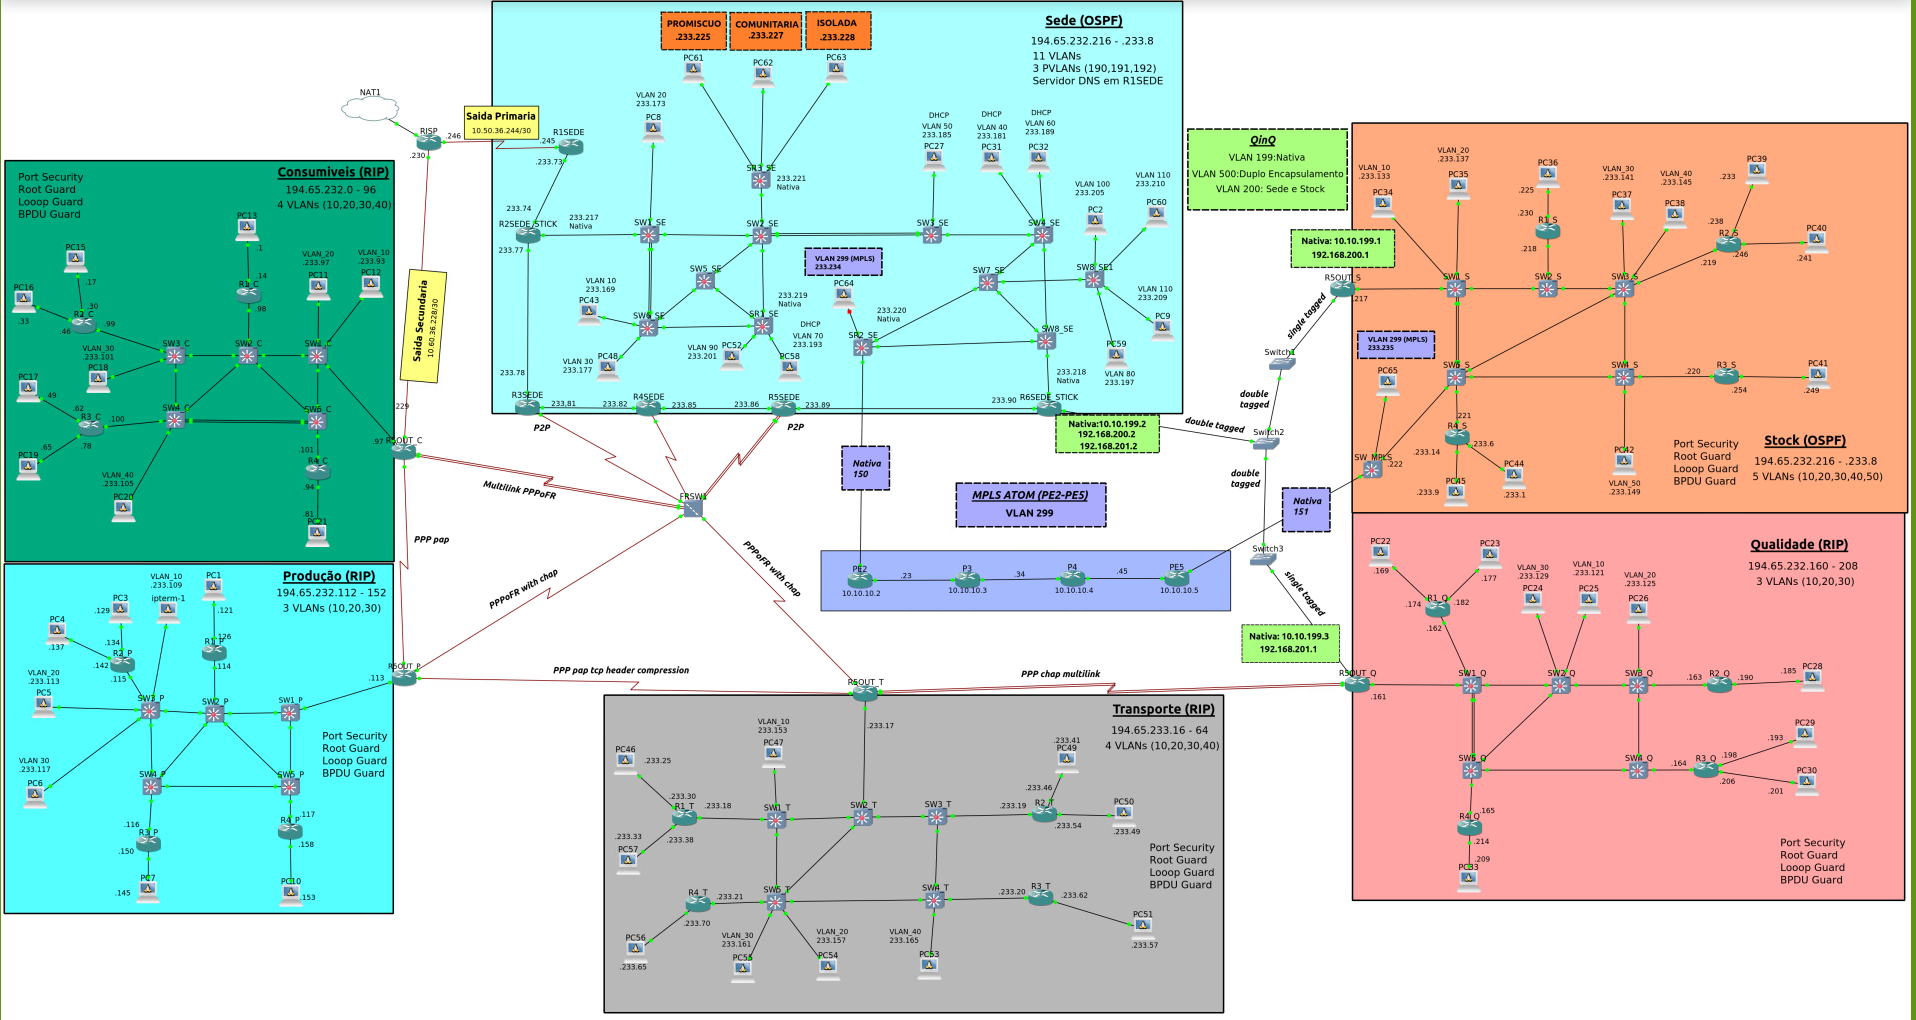
\includegraphics[width=1\textwidth]{topologia}
		\caption{Topologia}
		\label{fig.nav}
	\end{figure}
	
	\large
	\section{Endereçamento}
	\subsection{Endereçamento privado}
	\normalsize
    \paragraph{}
    O endereçamento privado foi usado maioritariamente para ligações entre routers de filiais diferentes para que o endereço público fornecido pelo ISP não fosse desperdiçado.
    O endereçamento privado foi usado no FrameRelay, PPP, MPLS e QinQ.


    \subsection{Endereçamento público}
    \normalsize
    \paragraph{}
    
    Foi usado VLSM no endereçamento público, fazendo com que cada \emph{link} de cada router representasse uma subrede diferente.\\
    O endereçamento atribuido pelo ISP foi o \textbf{194.65.232.0/22} sendo que o \textbf{194.65.233.0} também foi utilizado.
    
	
    \large
    \section{Filiais}
    \normalsize
    \paragraph{}
    Ao todo foram usados dois protocolos de encaminhamento (\textbf{RIP} e \textbf{OSPF}) fazendo a devida redistribuição de protocolos quando era necessário.
    Existe autenticação em todas as redes que usam o OSPF, sendo que no RIP optei por não usar autenticação.\\
    Todos os routers contêm uma única autenticação por \textbf{telnet} e é apresentado um \textbf{banner} aquando da entrada no mesmo.\\
    Em todas as filiais existem VLANs e existe tambem um terminal que comprova o bom funcionamento de todas elas.\\
    Foi usado o RSTP elegendo sempre a melhor  \textbf{Root Bridge} dependendo de cada filial, onde foi tambem configurado o \textbf{Port Security,Root Guard, Loop Guard e BPDU Guard}.\\
    O router de saída de cada filial representa um \textbf{Router on a stick} fazendo assim deste o \textbf{Default Gateway} das VLANs presentes naquela filial.

	\subsection{Consumíveis}
	\normalsize
	\paragraph{}
        Aqui foi usado o protocolo \textbf{RIP}. Esta filial contém 7 subredes e 4 VLANs.\\
        Foi também configurada uma \textbf{ligação secundária} ao RISP assim como \textbf{Multilink PPPoFR} com o R5Sede e \textbf{PPP pap} com o R5OUT da Produção. 

	\begin{figure}[h]
		\centering
		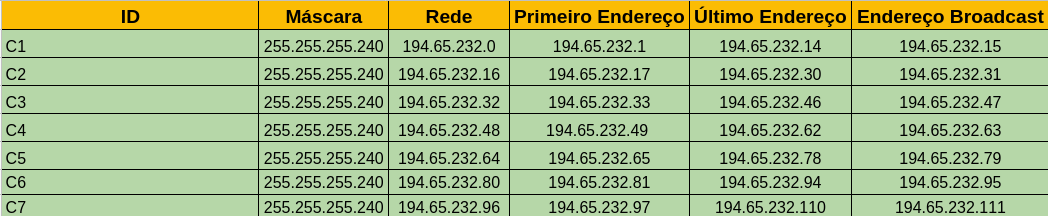
\includegraphics[width=0.9\textwidth]{vlsm-consumiveis}
		\caption{Subredes - Consúmiveis}
		\label{fig.nav}
              \end{figure}

              	\begin{figure}[h]
		\centering
		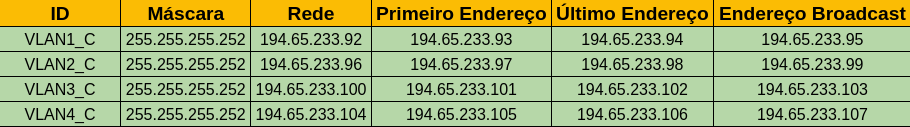
\includegraphics[width=0.9\textwidth]{vlsm-vlan-consumiveis}
		\caption{Vlans - Consúmiveis}
		\label{fig.nav}
	\end{figure}


	\pagebreak

	\subsection{Produção}
	\normalsize
	\paragraph{}
        Na Produção foi mais uma vez utilizado o \textbf{RIP}. Aqui existem 3 VLANs e 6 subredes sendo que mais uma vez o R5OUT\_P é o \textbf{Router on a stick} das VLANs.
        Aqui está configurado \textbf{PPP pap} com o R5OUT dos Consumíveis, \textbf{PPPoFR with chap} com o R3Sede e \textbf{PPP pap tcp header compression} com o R5OUT dos Transportes.

        \begin{figure}[h]
          \centering
          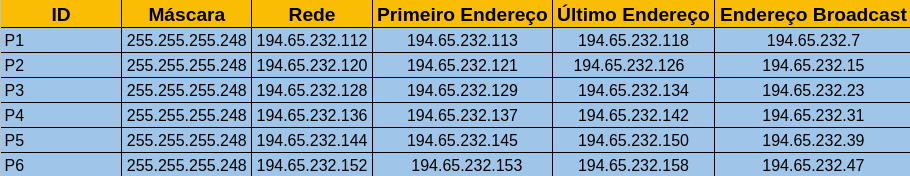
\includegraphics[width=0.9\textwidth]{vlsm-producao}
          \caption{Subredes - Produção}
          \label{fig.nav}
        \end{figure}

        \begin{figure}[h]
          \centering
          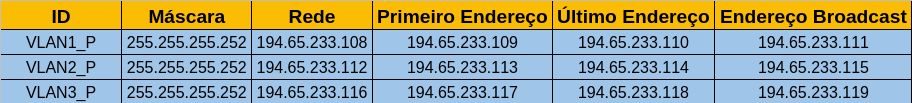
\includegraphics[width=0.9\textwidth]{vlsm-vlan-producao}
          \caption{Vlans - Produção}
          \label{fig.nav}
	\end{figure}

        \pagebreak
        
	\subsection{Transporte}
	\normalsize
	\paragraph{}
        Mais uma vez é utilizado o RIP como protocolo de encaminhamento dentro da empresa, e aqui existem 4 VLANs juntamente com 7 subredes. Aqui encontra-se configurado \textbf{PPP pap tcp header compression} com o R5OUT da Produção, \textbf{PPP chap multilink} com o R5OUT da Qualidade e \textbf{PPPoFR with chap} com o R4Sede.

        \begin{figure}[h]
          \centering
          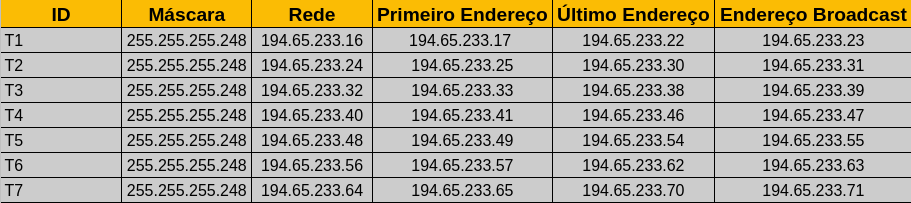
\includegraphics[width=0.9\textwidth]{vlsm-transporte}
          \caption{Subredes - Transporte}
          \label{fig.nav}
        \end{figure}

        \begin{figure}[h]
          \centering
          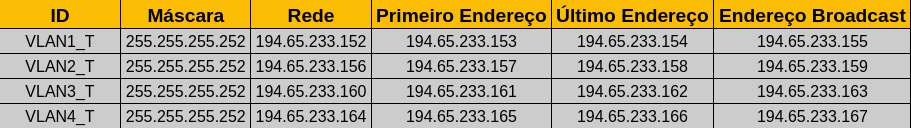
\includegraphics[width=0.9\textwidth]{vlsm-vlan-transporte}
          \caption{Vlans - Transporte}
          \label{fig.nav}
	\end{figure}


 	\subsection{Qualidade}
	\normalsize
	\paragraph{}
        Nesta filial encontra-se configurado o RIP e a mesma contêm 3 VLANs assim como 7 subredes.Esta filial tem uma ligação \textbf{PPP chap multilink} com o R5OUT dos Transportes e tem também uma \textbf{ligação QinQ} com o R6Sede.

        \begin{figure}[h]
          \centering
          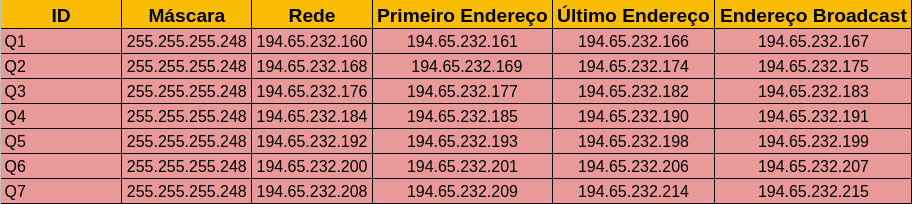
\includegraphics[width=0.9\textwidth]{vlsm-qualidade}
          \caption{Subredes - Qualidade}
          \label{fig.nav}
        \end{figure}

        \begin{figure}[h]
          \centering
          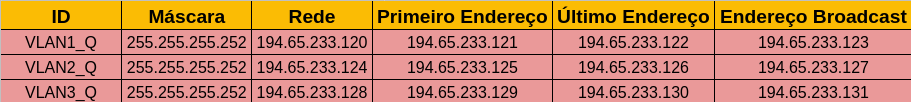
\includegraphics[width=0.9\textwidth]{vlsm-vlan-qualidade}
          \caption{Vlans - Qualidade}
          \label{fig.nav}
	\end{figure}

        \pagebreak
        
	\subsection{Stock}
	\normalsize
	\paragraph{}
        Nesta filial encontra-se configurado o \textbf{OSPF} com apenas uma área (\textbf{area 0}) e a mesma contêm 7 subredes e 5 VLANs. Aqui tambem existe uma \textbf{ligação QinQ} com o R6Sede assim como uma \textbf{ligação MPLS} com o SR2Sede.

        \begin{figure}[h]
          \centering
          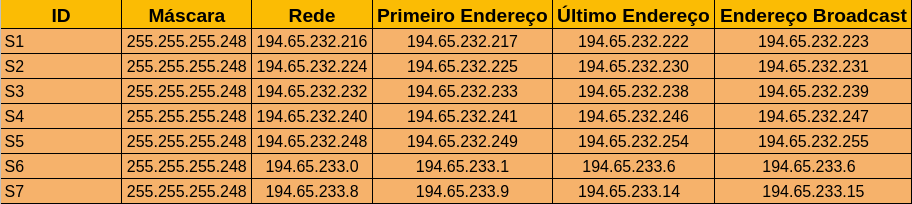
\includegraphics[width=0.9\textwidth]{vlsm-stock}
          \caption{Subredes - Stock}
          \label{fig.nav}
        \end{figure}

        \begin{figure}[h]
          \centering
          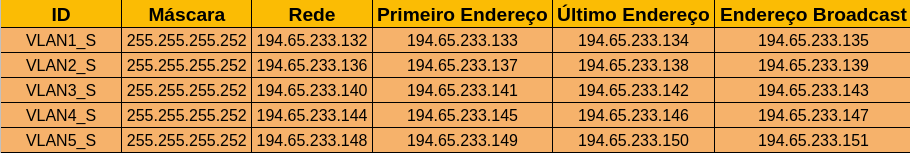
\includegraphics[width=0.9\textwidth]{vlsm-vlan-stock}
          \caption{Vlans - Stock}
          \label{fig.nav}
	\end{figure}


        \subsection{Sede}
        \normalsize
        \paragraph{}
        Na sede está configurado o protocolo \textbf{OSPF} apenas com uma área. Na sede existe então a ligação primária para o RISP, sendo esta a ligação prioritariamente utilizada aquando da saída para a Internet. Aqui existem 11 VLANs mais uma VLAN nativa, 3 Private Vlans e 5 subredes.\\
        Existem dois Routers on a stick (\textbf{R2SEDE\_STICK e R6SEDE\_STICK}) e três switch-routers (\textbf{SR1\_SE, SR2\_SE e SR3\_SE}) que são DGs de algumas VLANs.

        \begin{figure}[h]
          \centering
          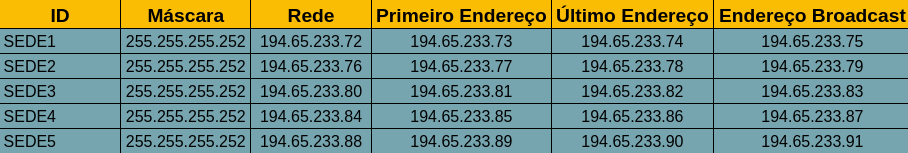
\includegraphics[width=0.9\textwidth]{vlsm-sede}
          \caption{Subredes - Sede}
          \label{fig.nav}
        \end{figure}

        \begin{figure}[h]
          \centering
          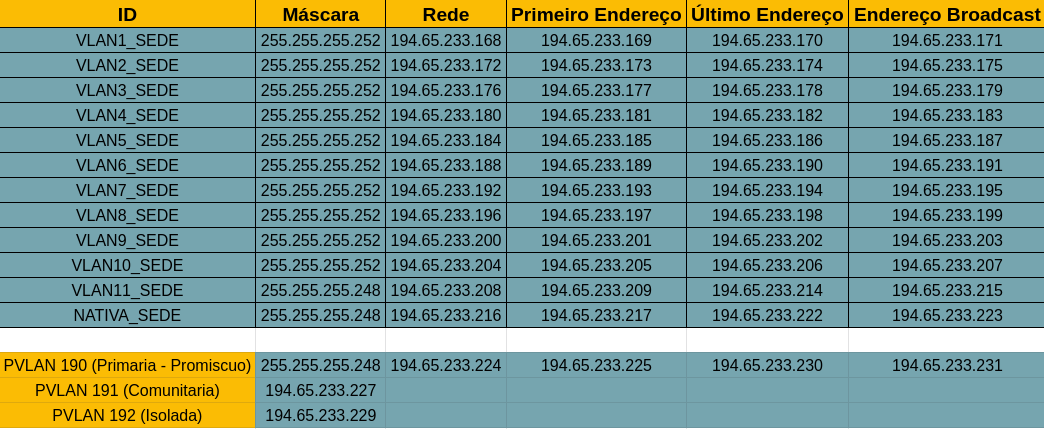
\includegraphics[width=0.9\textwidth]{vlsm-vlan-sede}
          \caption{Vlans - Sede}
          \label{fig.nav}
	\end{figure}

        \pagebreak
        
       	\large	
	\section{PVLANs}
	\normalsize
	\paragraph{}
        Na sede foi criada uma \textbf{Private VLAN (190)} de modo a implementar um requisito do trabalho. Esta VLAN divide-se em duas sendo que a PVLAN 191 é do tipo \textbf{Community} e a PVLAN 192 é do tipo \textbf{Isolated}. O DG da mesma é o switch-router \textbf{SR3\_SE}.


	\large	
	\section{FrameRelay}
	\normalsize
	\paragraph{}
        O FrameRelay foi utilizado para interligar filias entre si e para também conseguir interligar a sede com algumas filiais de modo a cumprir mais um requisito pedido no trabalho prático. Para as ligações foram utilizadas várias maneiras de autenticação como por exemplo o \textbf{PPPoFR with chap} e tambem o \textbf{Multilink PPPoFR}.

        \begin{figure}[h]
          \centering
          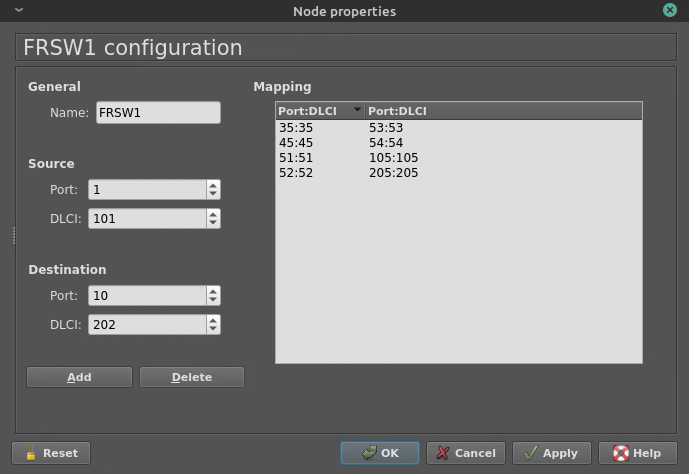
\includegraphics[width=0.6\textwidth]{frame-relay}
          \caption{FrameRelay}
          \label{fig.nav}
	\end{figure}


	\pagebreak

	\large	
	\section{QinQ}
	\normalsize
        \paragraph{}
        O QinQ foi usado para interligar a Sede com o Stock e com a Qualidade sendo que tanto o Stock como a Qualidade conseguem comunicar entre si pois apenas é usada uma VLAN para o duplo encapsulamento sendo esta a \textbf{VLAN 500}. Foi criada então a VLAN 199 sendo esta a nativa entre R6Sede, R5OUT\_S e R5OUT\_Q. Depois foi criada uma subrede entre o R6Sede e o R5OUT\_S e outra subrede entre o R6Sede e o R5OUT\_Q. Depois de configurado o QinQ foi possível haver comunicação entre filiais e de filiais para a Sede a partir do QinQ.

        \large	
	\section{MPLS - ATOM}
	\normalsize
        \paragraph{}
        O MPLS foi usado para interligar o Stock com a Sede. No MPLS foi usado o mecanismo ATOM na \textbf{VLAN 299} onde é feita a ligação entre o \textbf{PE2} e o \textbf{PE5}. Depois existe uma VLAN Nativa entre o SR2\_SE e o PE2 sendo esta a \textbf{VLAN 150} e outra nativa entre o PE5 e o SW\_MPLS sendo esta a \textbf{VLAN 151}.\\ Por fim foi colocado um terminal na sede com a VLAN 299 e outro terminal no Stock na VLAN 299 onde ambos conseguem comunicar sem qualquer problema.

        \begin{figure}[h]
          \centering
          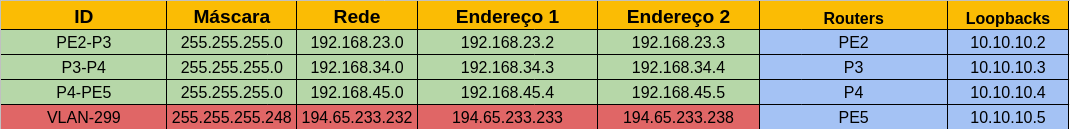
\includegraphics[width=0.9\textwidth]{mpls}
          \caption{MPLS - ATOM}
          \label{fig.nav}
	\end{figure}



    \pagebreak
	\large
	\section{Conclusão}
	\normalsize
	\paragraph{}
	No fim todos os objetivos propostos no enunciado do trabalho foram conseguidos fazendo com que fossem aplicados todos os conhecimentos e técnicas aprendidas e praticadas tanto nas aulas práticas como nas aulas teóricas da cadeira de tecnologias de ligação.

\end{document}